\subsection{Simulation}

\begin{frame}
\begin{center}
	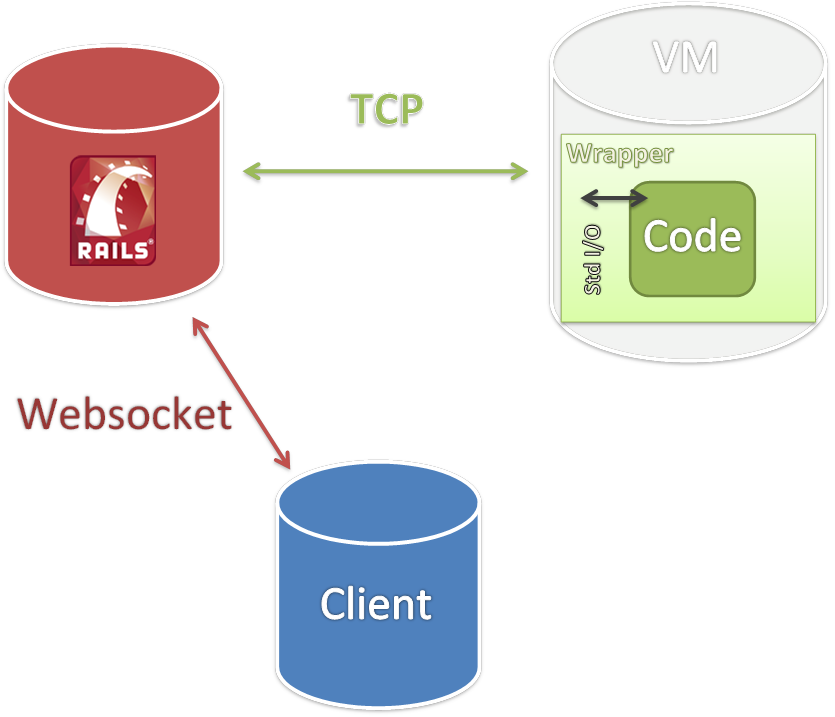
\includegraphics[scale=0.35]{overview}
\end{center}
\end{frame}

\begin{frame}
	\begin{center}
		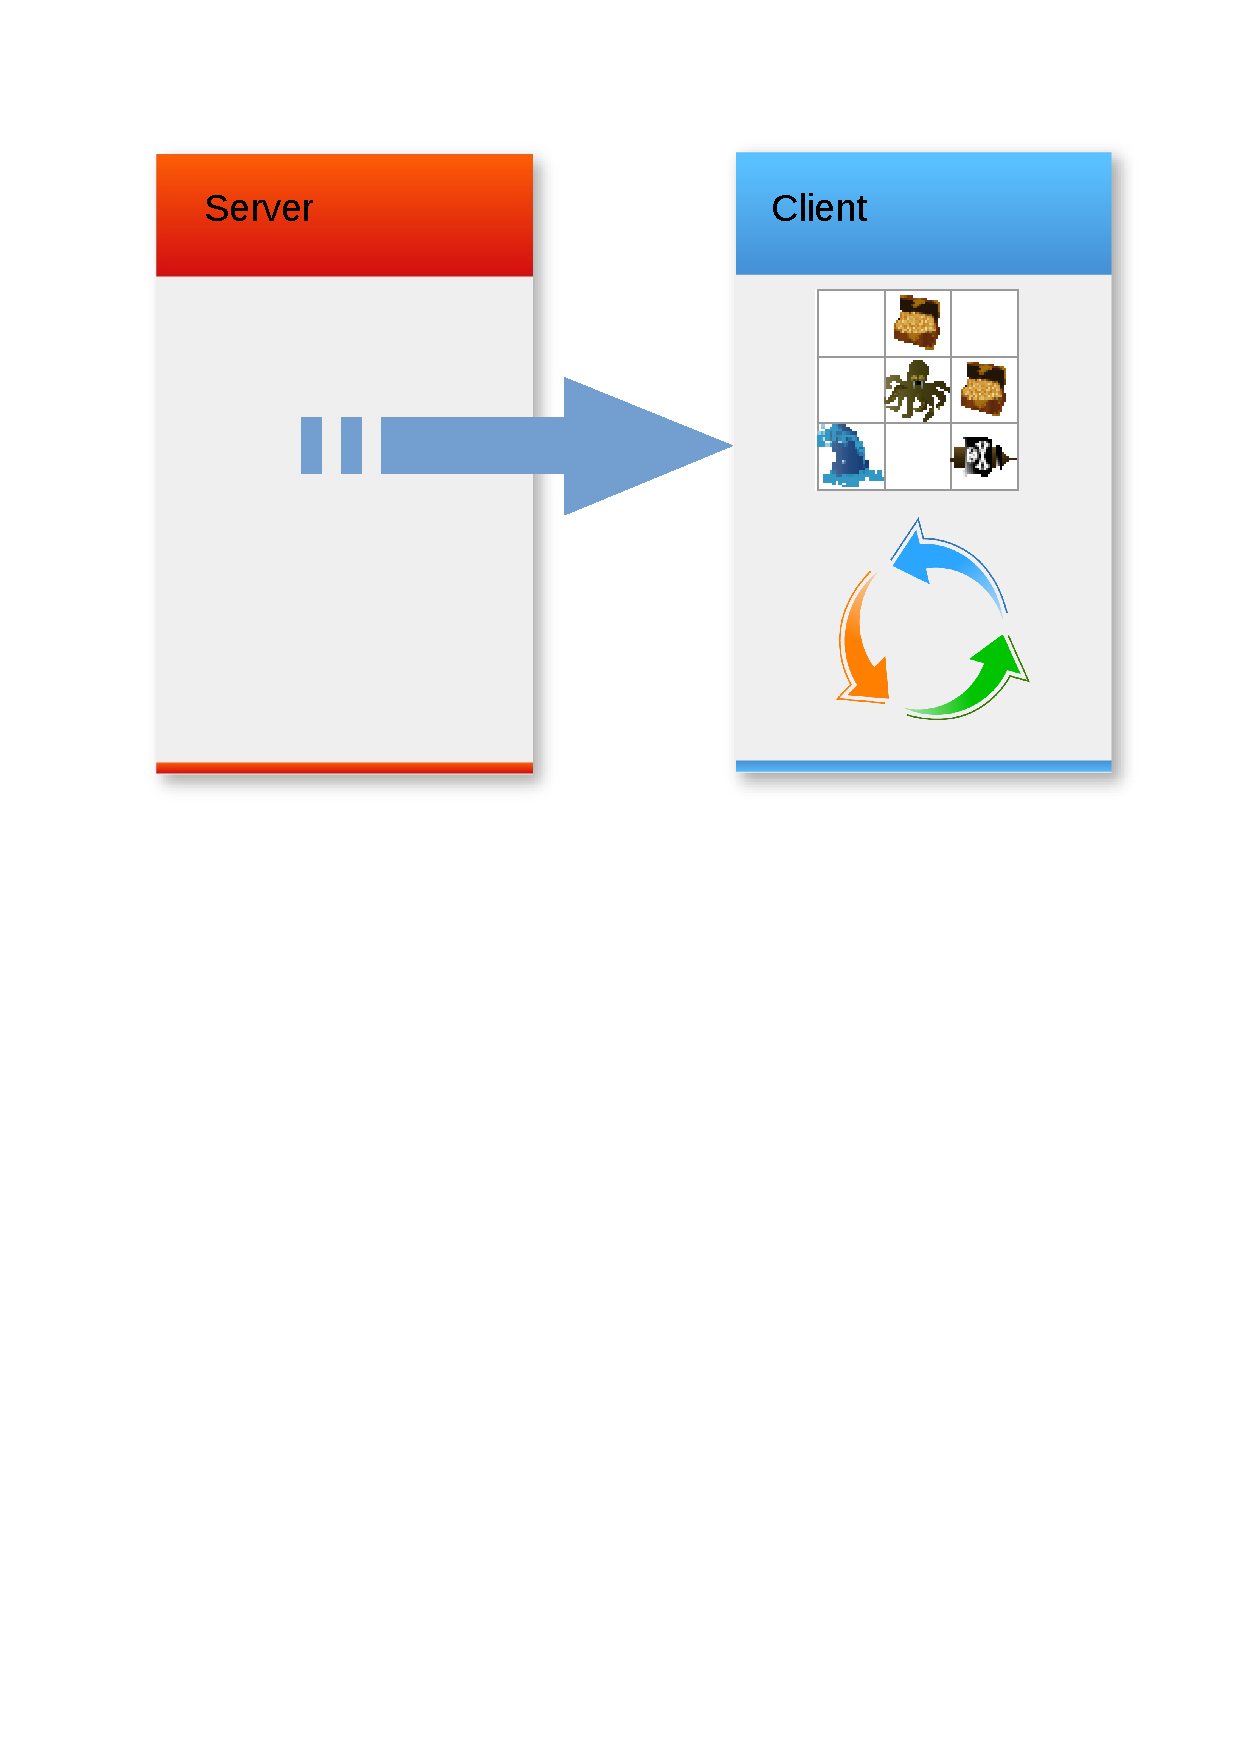
\includegraphics[scale=0.5]{simulation/Simulation1.pdf}
	\end{center}
	%Am Anfang hatten wir gedacht, dass wir die Simulation auf dem Client laufen lassen, damit der Server entlastet wird. 
	
	%Wir haben versucht, die Simulation möglichst Serverlastig zu gestalten. So Liegt auf dem Server das Grid mit allen Objekten. Da die GUI beim Starten der Simulation das Grid mit dem Objekten an den Server sendet, stimmen am Anfang Grid auf Server und Client überein. Es werden nur Änderungen und wichtige Informationen übermittelt. Bei put z.B nur das hinzugefügte Objekt mir Koordinaten, bei look nur das zu highlightende Feld.
\end{frame}

\begin{frame}
	\begin{center}
		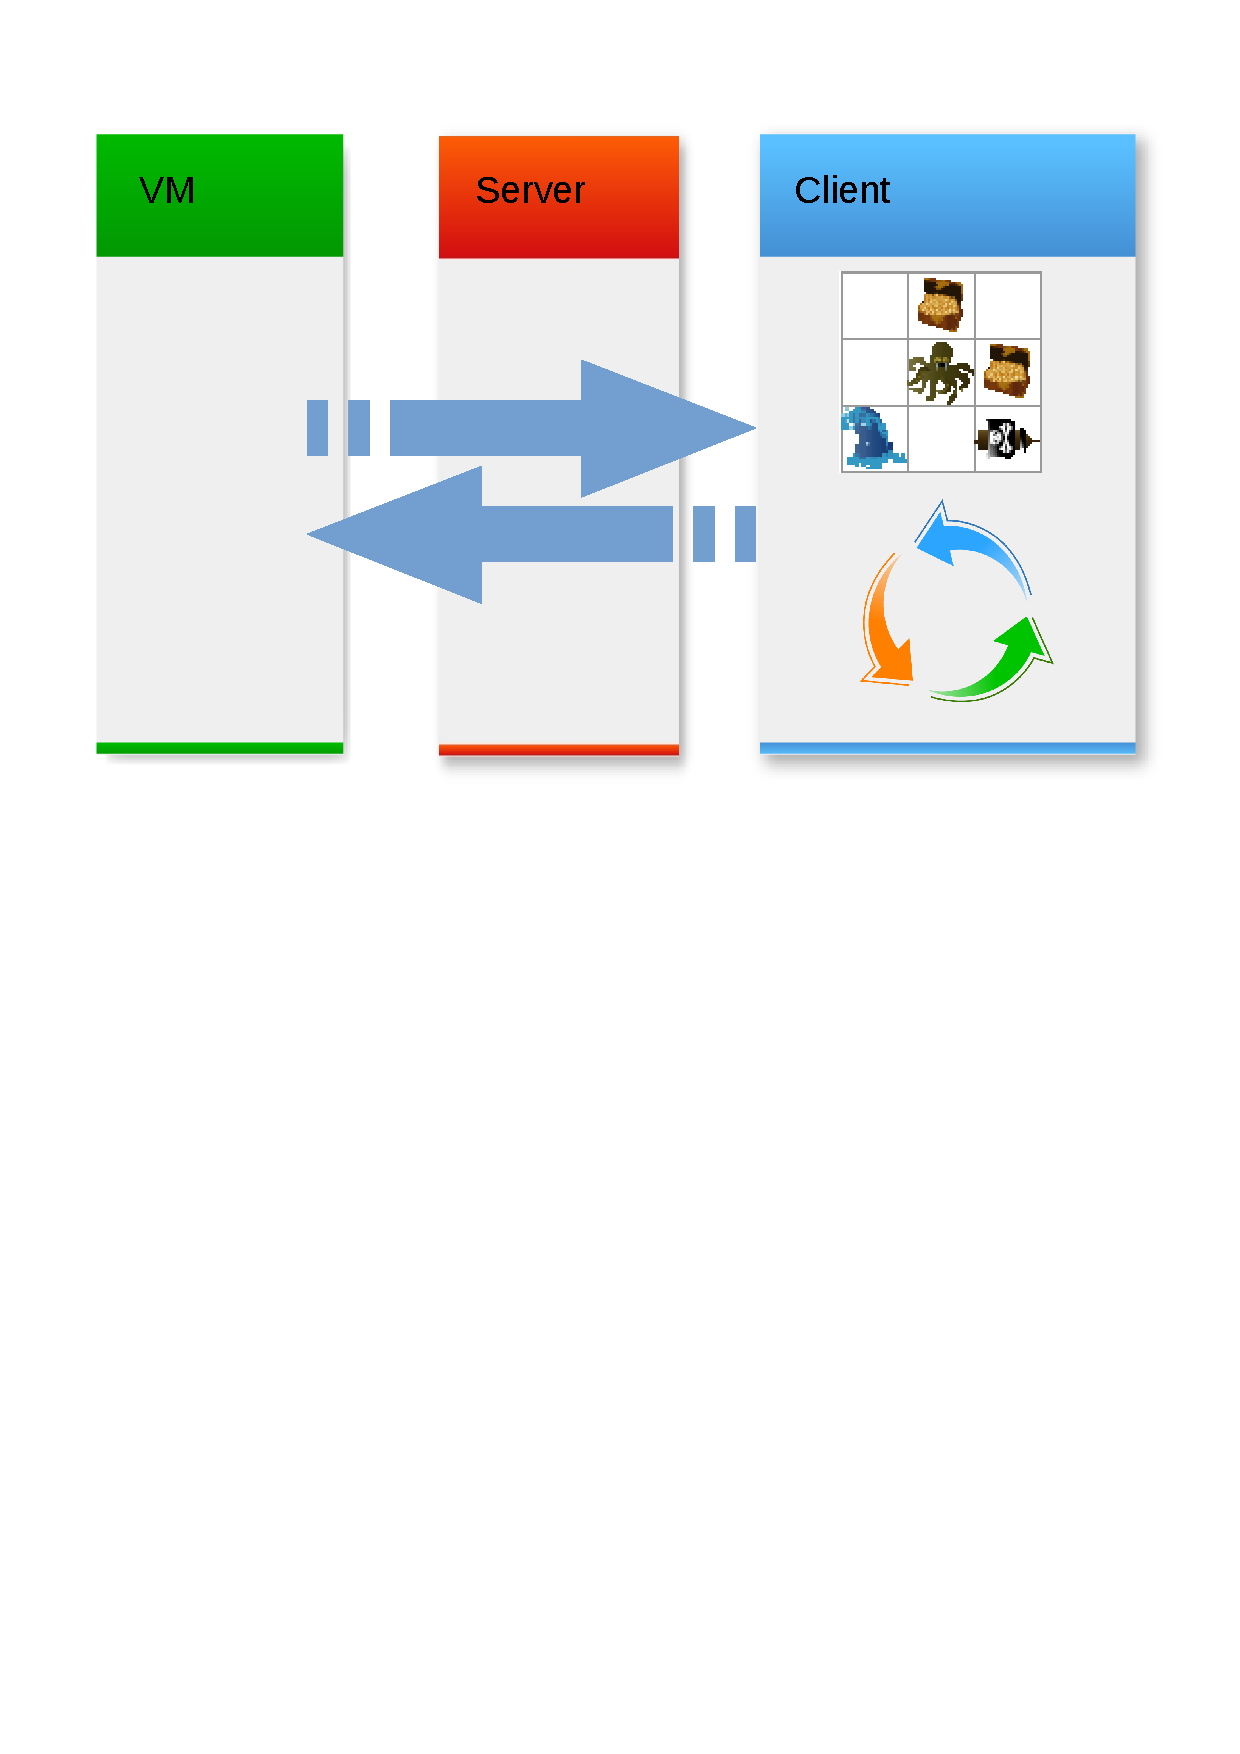
\includegraphics[scale=0.5]{simulation/Simulation2.pdf}
	\end{center}
	%Aber da der Fall auftreten kann, dass die VM auf eine Antwort der look Funktion wartet, müsste der Client über den Server den Rückgabewert an die VM senden. Die VM müsste dann auf die Simulation auf dem Client warten.
\end{frame}

\begin{frame}
	\begin{center}
		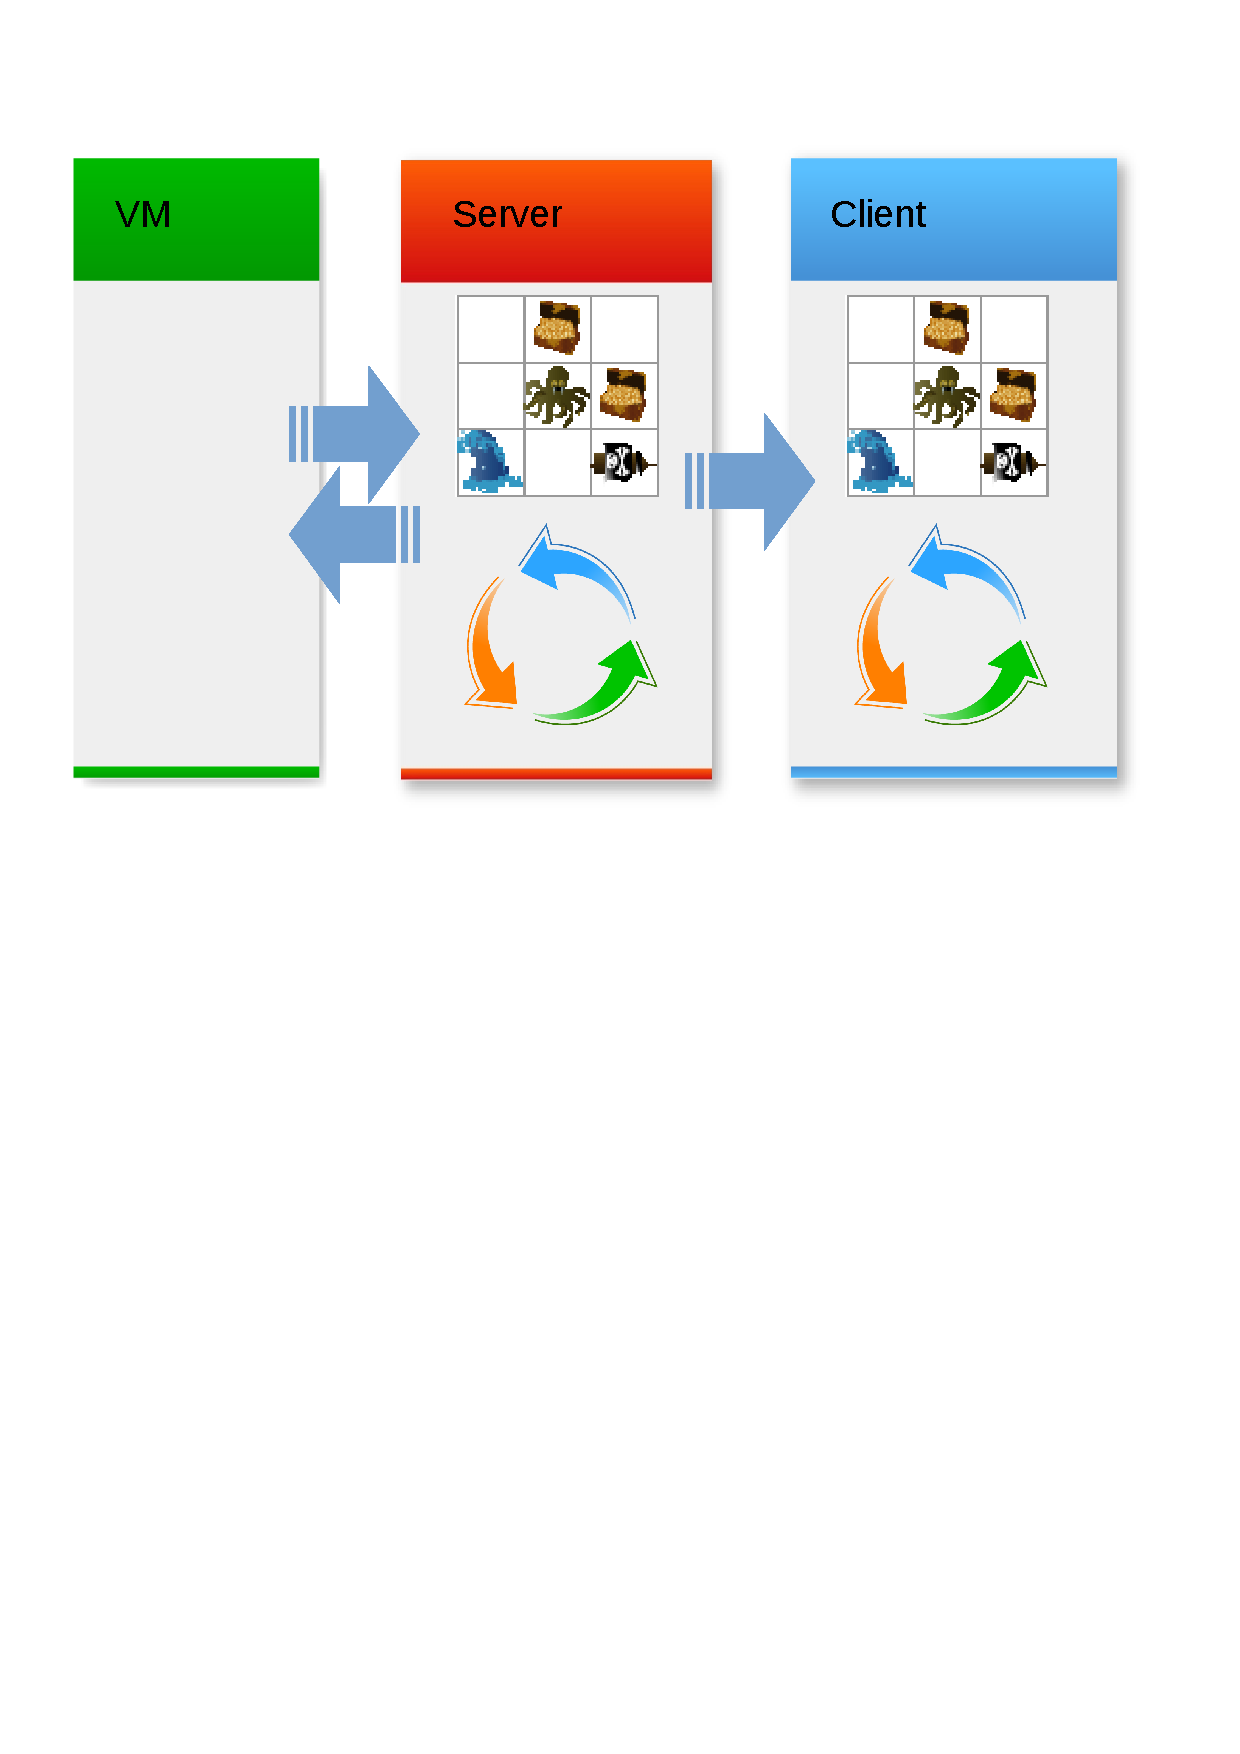
\includegraphics[scale=0.5]{simulation/Simulation3.pdf}
	\end{center}
	%Um das zu umgehen, brauchen wir also auch auf dem Server
\end{frame}

\begin{frame}
	\begin{center}
		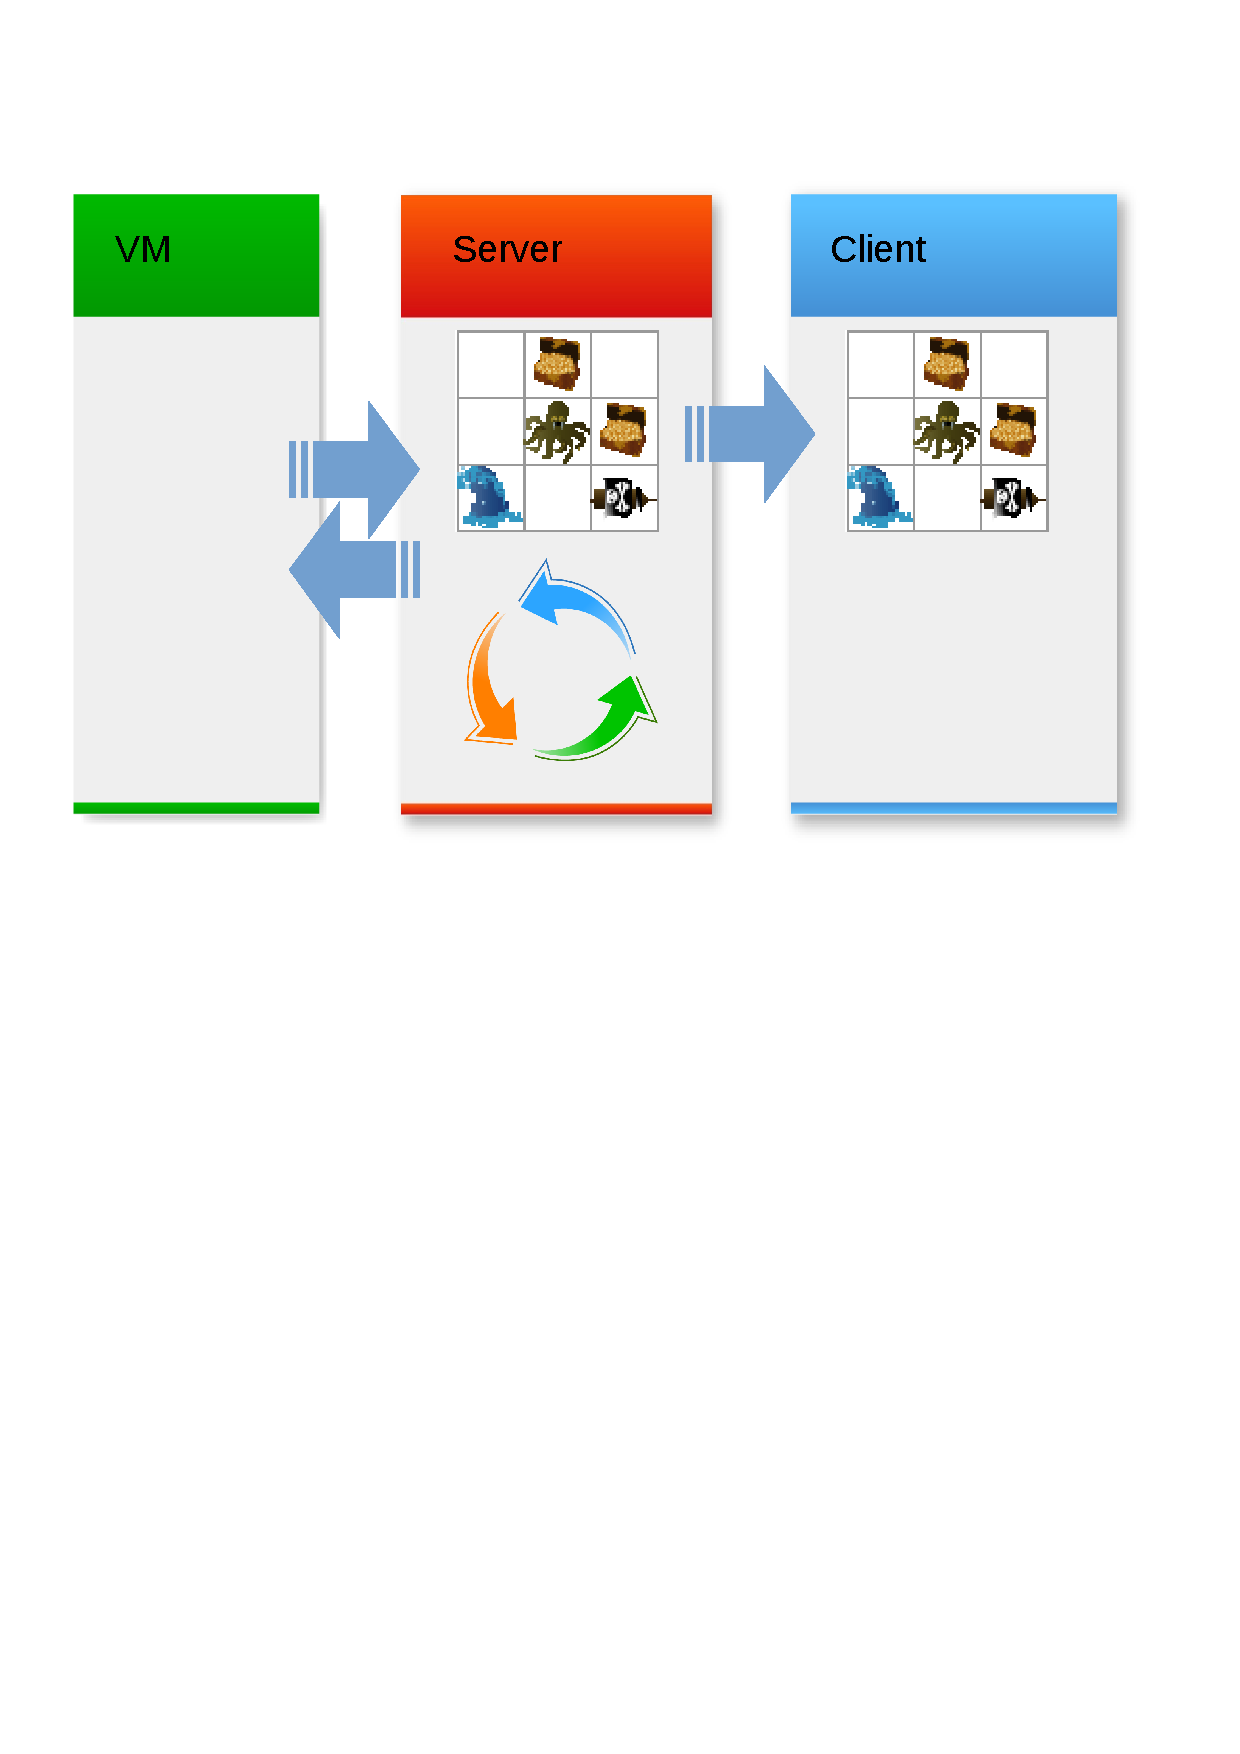
\includegraphics[scale=0.5]{simulation/Simulation4.pdf}
	\end{center}
	% Am Anfang sind Grid auf Server und auf Client identisch, da Client sein Grid an den Server sendet. Bei der Simulation werden nur noch die Änderungen an den Client gesendet.
\end{frame}

\begin{frame}
	\begin{center}
		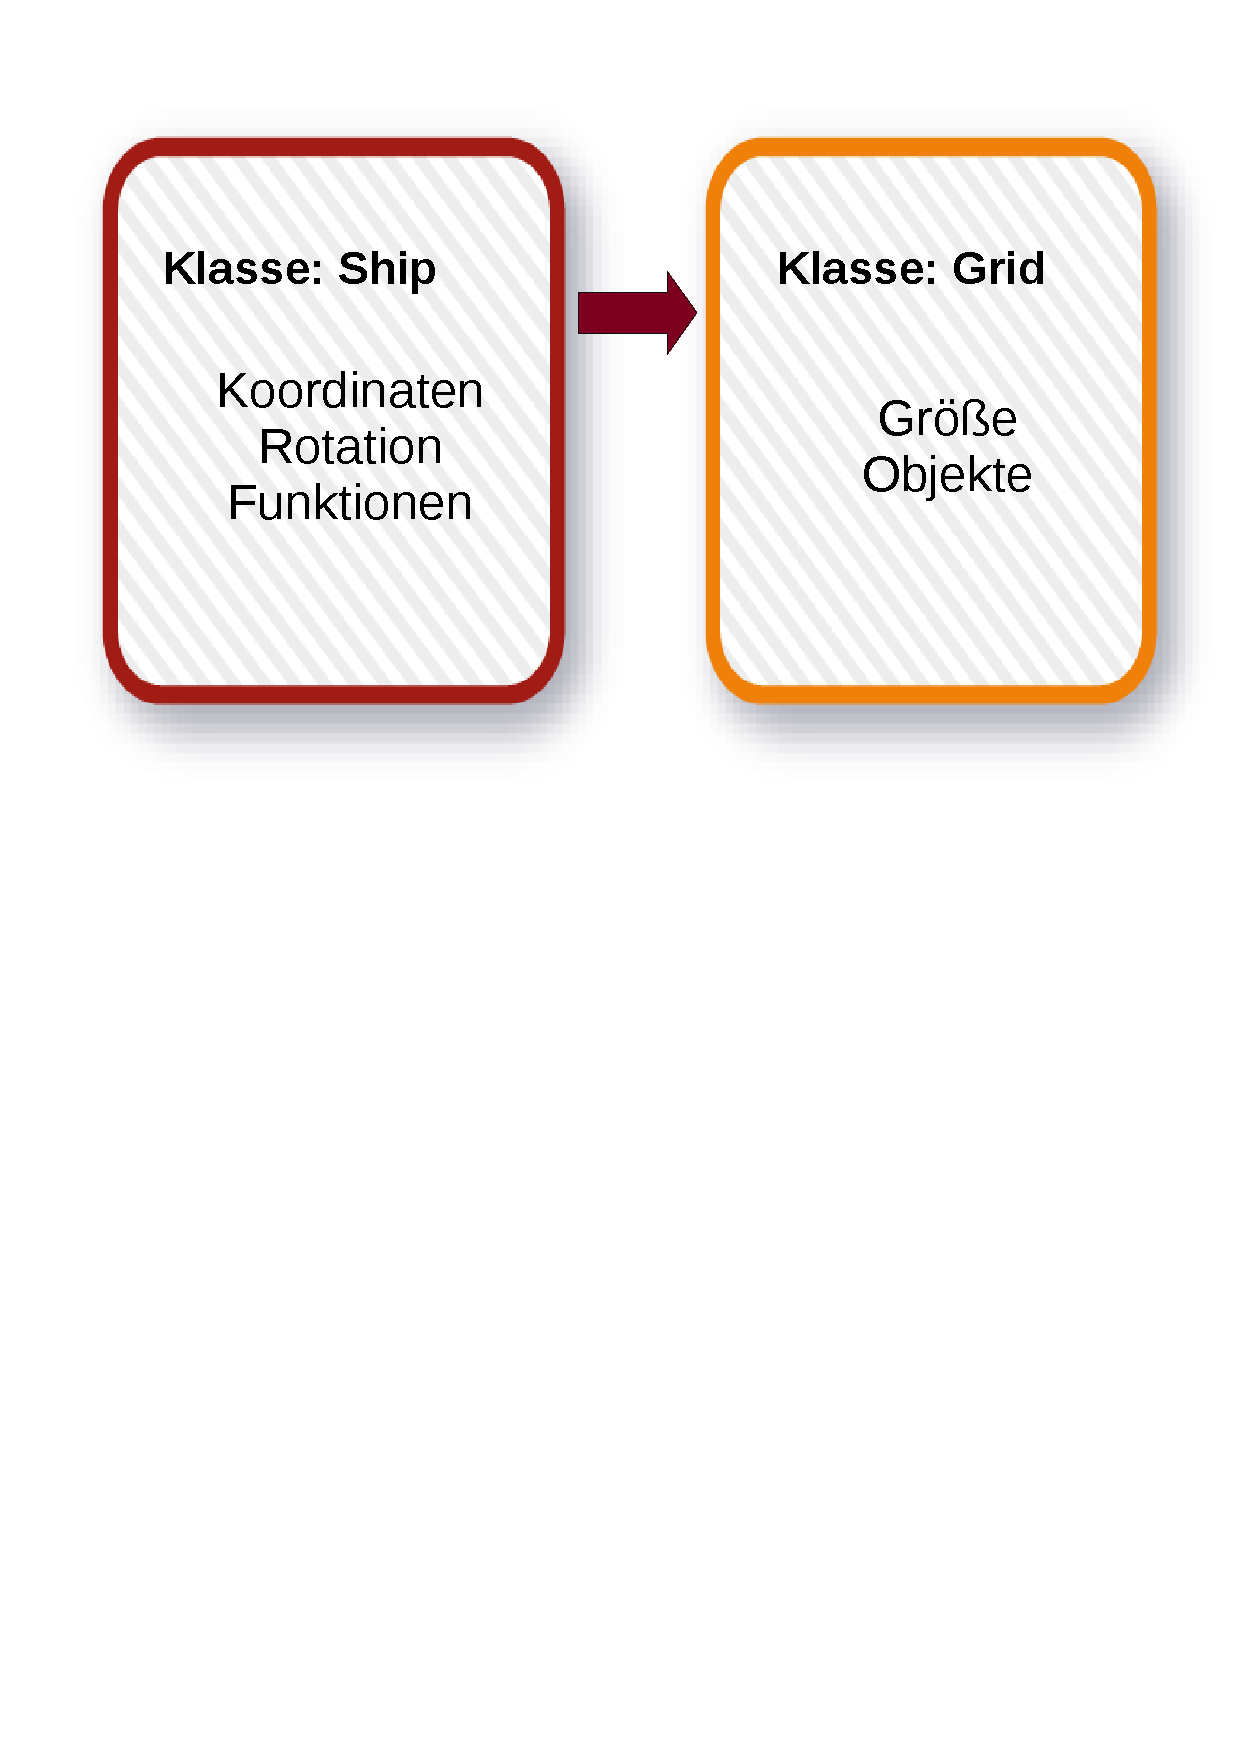
\includegraphics[scale=0.5]{simulation/Simulation5.pdf}
	\end{center}
	%Wir speichern alle Objecte in einem zweidimensionalen Hash, will man auf eine nicht definierte Koordinate zugreifen, bekommt man als Object :nothing zurück. Das Schiff wird seperat als eigenständige Klasse gespeichert und hier befinden sich auch die sich auf das Schiff beziehenden Funktionen. Zusätzlich zu den Koordinaten besitzt das Schiff auch eine Rotation. Jede Funktion 
\end{frame}

\begin{frame}
	\inputminted[linenos, frame=lines, label= functions]{ruby}		{simulation/first.rb}
%Wir haben hier eine Liste von Funktionen. Wenn die VM etwas an den Server sendet, wird in der Liste überprüft, was man damit machen soll. Mit Unterstrich kann man der Funktion noch Atribute mitgeben. Es gibt einmal die Funktionen für die Simulation und dann noch Funktionen für weitere Informationen. 
	\ \\
	$turn\_ right \rightarrow @ship.turn!(:right)$
\end{frame}

\begin{frame}
	\begin{center}
		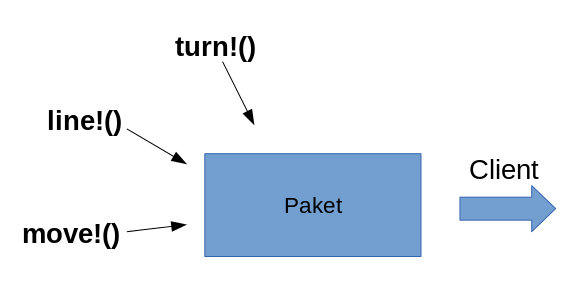
\includegraphics[scale=0.5]{simulation/Pakete.jpg}
	\end{center}
	%Für jede Zeile des ursprünglichen Codes wird ein Paket gepackt, in die jede aufgerufene Funktion Informationen für den Server packen können. Ist man am Ende einer Zeile angelangt, wird das Paket losgeschickt. 
\end{frame}


\begin{frame}
	\begin{center}
		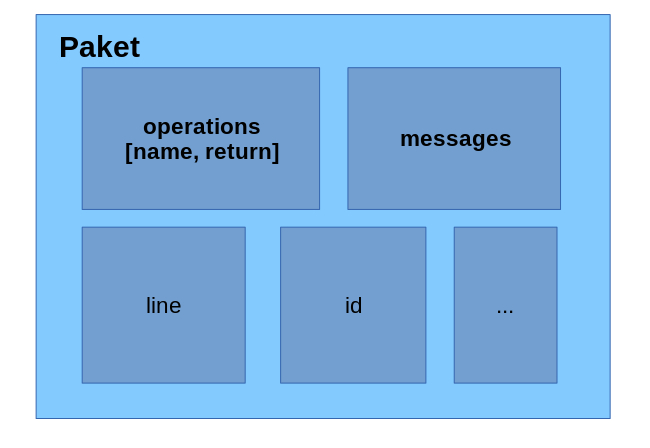
\includegraphics[scale=0.5]{simulation/Pakete2.jpg}
	\end{center}
	%Wir stellen verschiedene Paketschlüssel zur verfügung, am wichtigsten für die Simulation ist message und operations. Über Operations werden Funktionen beim Client aufgerufen und mit Message werden Nachrichten an den User übergeben.
\end{frame}


\begin{frame}
	\begin{itemize}
		\item Grid auf Server und Client sind identisch
		\item Nur Änderungen des Grids werden dem Client gesendet
	\end{itemize}
\end{frame}